\subsection*{Problema 35}

\textbf{Enunciado:}
Calcular la integral indefinida:
\begin{equation*}
\int \dfrac{2x^2 + 41x - 91}{x^3 - 2x^2 - 11x + 12} \, dx
\end{equation*}

\textbf{Solución:}
El denominador se puede factorizar como se indica en las observaciones:
\begin{equation*}
x^3 - 2x^2 - 11x + 12 = (x - 1)(x - 4)(x + 3)
\end{equation*}

Planteamos la descomposición en fracciones simples para el integrando:
\begin{multline*}
\dfrac{2x^2 + 41x - 91}{(x - 1)(x - 4)(x + 3)} = \\
\dfrac{A}{x - 1} + \dfrac{B}{x - 4} + \dfrac{C}{x + 3}
\end{multline*}

Multiplicando ambos lados por el denominador común, obtenemos:
\begin{multline*}
2x^2 + 41x - 91 = A(x - 4)(x + 3) \\
+ B(x - 1)(x + 3) + C(x - 1)(x - 4)
\end{multline*}

Evaluamos en los valores críticos para hallar las constantes:
\begin{align*}
\text{Si } x &= 1: \\
2(1)^2 + 41(1) - 91 &= A(1 - 4)(1 + 3) \\
-48 &= -12A \implies A = 4 \\
\text{Si } x &= 4: \\
2(4)^2 + 41(4) - 91 &= B(4 - 1)(4 + 3) \\
84 &= 21B \implies B = 4 \\
\text{Si } x &= -3: \\
2(-3)^2 + 41(-3) - 91 &= C(-3 - 1)(-3 - 4) \\
-196 &= 28C \implies C = -7
\end{align*}

Sustituyendo los valores de $A$, $B$ y $C$ en la integral:
\begin{multline*}
\int \dfrac{2x^2 + 41x - 91}{x^3 - 2x^2 - 11x + 12} \, dx = \\
\int \left( \dfrac{4}{x - 1} + \dfrac{4}{x - 4} - \dfrac{7}{x + 3} \right) dx
\end{multline*}

Integramos cada término de forma directa utilizando logaritmos:
\begin{align*}
\int \dfrac{4}{x - 1} \, dx &= 4 \ln|x - 1| \\
\int \dfrac{4}{x - 4} \, dx &= 4 \ln|x - 4| \\
\int \dfrac{7}{x + 3} \, dx &= 7 \ln|x + 3|
\end{align*}

Agrupando los resultados y aplicando propiedades de logaritmos, la solución general es:
\begin{multline*}
= 4 \ln|x - 1| + 4 \ln|x - 4| \\
- 7 \ln|x + 3| + C
\end{multline*}
O de forma compacta:
\begin{equation*}
= \ln\left( \dfrac{(x - 1)^4 (x - 4)^4}{(x + 3)^7} \right) + C
\end{equation*}

\begin{figure}[H]
	\centering
	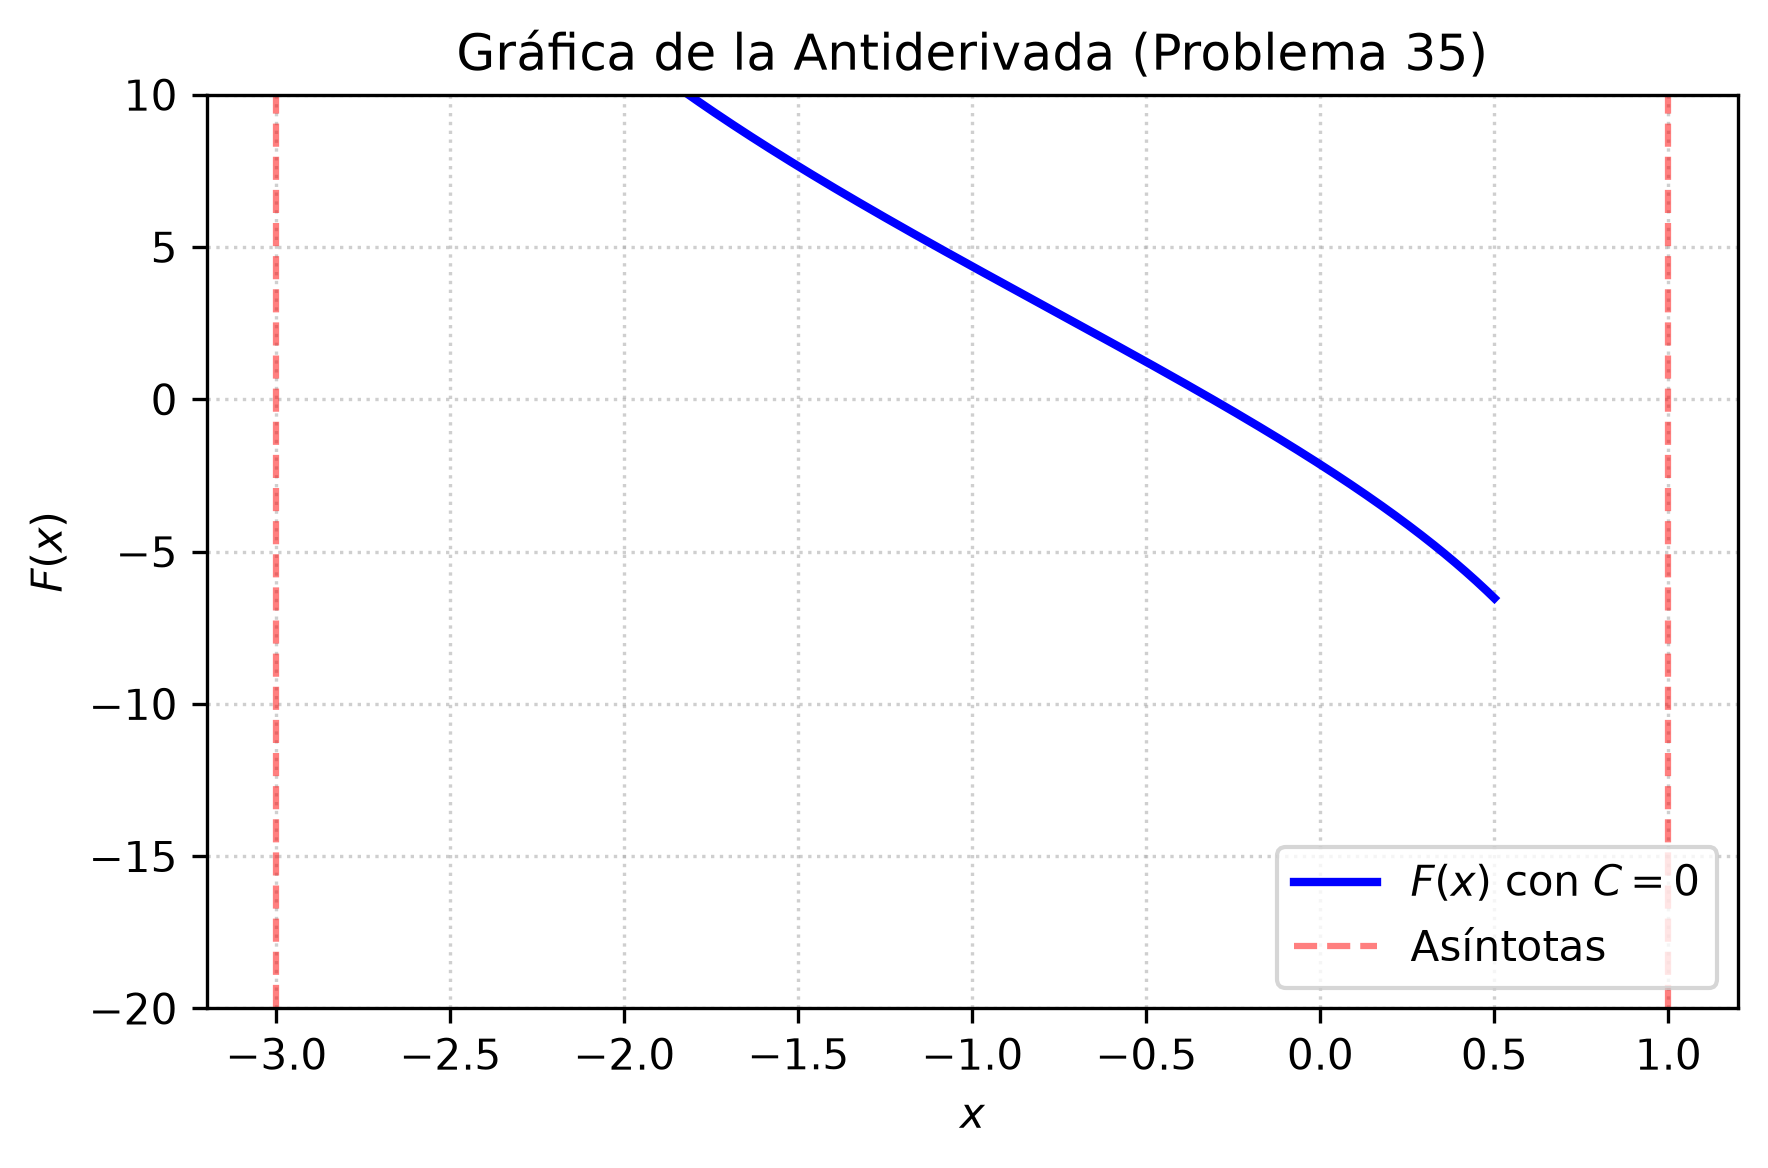
\includegraphics[width=\columnwidth]{semana_03/graficas/SEM03_P35_grafica.png}
	\caption{Representación gráfica de $f(x)$ y su antiderivada $F(x)$ evaluada para la constante de integración $C = 0$ (Problema 35).}
	\label{fig:problema35}
\end{figure}
